% This must be in the first 5 lines to tell arXiv to use pdfLaTeX, which is strongly recommended.
\pdfoutput=1
% In particular, the hyperref package requires pdfLaTeX in order to break URLs across lines.

\documentclass[11pt]{article}

% Remove the "review" option to generate the final version.
% \usepackage[review]{emnlp2021}
\usepackage{emnlp2021}

% Standard package includes
\usepackage{times}
\usepackage{latexsym}

% For proper rendering and hyphenation of words containing Latin characters (including in bib files)
\usepackage[T1]{fontenc}

% This assumes your files are encoded as UTF8
\usepackage[utf8]{inputenc}
\usepackage{microtype}

% ======================================================================
% PEC For some reason the EMNLP templates put LH column line numbers on
% the right side. This switches them to the left side.
\usepackage[switch]{lineno} % default option is 'left
% ======================================================================

% PEC additions
\usepackage{graphicx}
\usepackage{amsmath}   % for \begin{align}
\newcommand{\nk}[1]{\textcolor{green}{Nora: #1}}
\newcommand{\reworded}[1]{\textcolor{blue}{#1}}
\newcommand{\eat}[1]{}
\newcommand{\red}[1]{\textcolor{red}{#1}}
\newcommand{\blue}[1]{\textcolor{blue}{#1}}
\newcommand{\orange}[1]{\textcolor{orange}{#1}}
\newcommand{\green}[1]{\textcolor{ForestGreen}{#1}}
\newcommand{\teal}[1]{\textcolor{teal}{#1}}
\newcommand{\magenta}[1]{\textcolor{magenta}{#1}}
\usepackage{quoting}
\newenvironment{myquote}{                   % list without par spacings
  \parskip 0mm \begin{quoting}[vskip=0mm,leftmargin=2mm]}{
\end{quoting}}
\newenvironment{myquote2}{                   % list without par spacings
  \parskip 1mm \begin{quoting}[vskip=0mm,leftmargin=4mm]}{
\end{quoting}}
\newenvironment{ite}{                     % list without par spacings
     \parskip 0cm \begin{itemize} \parskip 0cm \parsep 0cm \itemsep 0cm \topsep 0cm}{
        \end{itemize}} %  \parskip 0cm}
\newenvironment{enu}{                   % list without par spacings
     \parskip 0cm \begin{list}{}{\parsep 0cm \itemsep 0cm \topsep 0cm}}{
       \end{list}} %  \parskip 0cm}
\newenvironment{des}{                 % list without par spacings
     \parskip 0cm \begin{list}{}{\parsep 0cm \itemsep 0cm \topsep 0cm}}{
       \end{list}} %  \parskip 0cm}
\newenvironment{myenumerate}{                   % list without par spacings
     \parskip 0cm \begin{enumerate}{\parsep 0cm \itemsep 0cm \topsep 0cm}}{
        \end{enumerate}} %  \parskip 0cm}
\newenvironment{myitemize}{                     % list without par spacings
     \parskip 0cm \begin{itemize}{\parsep 0cm \itemsep 0cm \topsep 0cm}}{
        \end{itemize}} %  \parskip 0cm}

% ======================================================================

% If the title and author information does not fit in the area allocated, uncomment the following
%
%\setlength\titlebox{<dim>}
%
% and set <dim> to something 5cm or larger.

\title{Enriching a Model's Notion of Belief using a Persistent Memory} 
% BeliefBanks: Adding Persistent Memory to Enrich a Model's Notion of Belief (?) \\
% What does My Model Believe? }

% Author information can be set in various styles:
% For several authors from the same institution:
% \author{Author 1 \and ... \and Author n \\
%         Address line \\ ... \\ Address line}
% if the names do not fit well on one line use
%         Author 1 \\ {\bf Author 2} \\ ... \\ {\bf Author n} \\
% For authors from different institutions:
% \author{Author 1 \\ Address line \\  ... \\ Address line
%         \And  ... \And
%         Author n \\ Address line \\ ... \\ Address line}
% To start a seperate ``row'' of authors use \AND, as in
% \author{Author 1 \\ Address line \\  ... \\ Address line
%         \AND
%         Author 2 \\ Address line \\ ... \\ Address line \And
%         Author 3 \\ Address line \\ ... \\ Address line}

\author{Nora Kassner\textsuperscript{1,2},  Oyvind Tafjord\textsuperscript{1}, Hinrich Sch{\"u}tze\textsuperscript{2}, Peter Clark\textsuperscript{1} \\
\textsuperscript{1}Allen Institute for AI, Seattle, WA \\
\textsuperscript{2}Center for Information and Language Processing, 
LMU Munich, Germany \\
\texttt{kassner@cis.lmu.de} \\
\texttt{\{oyvindt,peterc\}@allenai.org} 
}

\begin{document}
\maketitle
\begin{abstract}
% \nk{Regarding the title: I liked the Believe me...}
Although pretrained language models (PTLMs) have been shown to contain significant
amounts of world knowledge, they can still produce inconsistent answers to questions when probed,
even after using specialized training techniques to reduce inconsistency. As a result, it can be
hard to identify what the model actually
"believes" about the world. Our goal is to reduce this problem, so systems are 
more globally consistent and accurate in their answers. Our approach is to add a
memory component - a BeliefBank - that records a model's answers,
and two mechanisms that use it to improve consistency among beliefs. First, a reasoning
component - a weighted SAT solver - improves consistency by flipping
answers that significantly clash with others. Second, a feedback
component re-queries the model but using known beliefs as context.
We show that, in a controlled experimental setting, these two mechanisms
improve both accuracy and consistency. This is significant as it is a
first step towards endowing models with an evolving memory,
allowing them to construct a more coherent picture of the world.\footnote{Dataset is available at https://allenai.org/data/beliefbank}
\end{abstract}

\eat{
\red{Why experiments are slow:
\begin{itemize}
    \item calibration is a problem!!! When I extended the dataset the calibration seems to not work well. I changed it to a heuristic alternative which seems to work but that means I have to rerun all SAT solving experiments
    \item SAT solving takes per entity: 6 min
    \item each run of the full graph takes > 1h
    \item + 10 plants: 10 h
    \item + 20 incremental with random context: 20
    \item + 20 incremental with bm25 context: 20
    \item + 20 incremental with bm25 SAT solved context: 20
    \item + averaging over multiple splits maybe 5?: 20*4
\end{itemize}}

\red{What are the current issues:
\begin{itemize}
    \item If calibration is of F1 can still improve but it flips essential things from no-->yes and random things from yes-->no
    \item What kind of F1 should I report? Derivable facts (small test set but large improvements), gold facts (even smaller test set with good model performance and only small improvements, all IsA facts (might include a couple of wrong labels, large test set, only slight improvements as many nodes need more mutual exclusive connectivity)
    \item I have to filter plurals
    \item Do we expect the model to understand negation inside to context window?
\end{itemize}}
}

\section{Introduction}

% \vspace{-1mm}
\begin{figure}[t]
\centering
     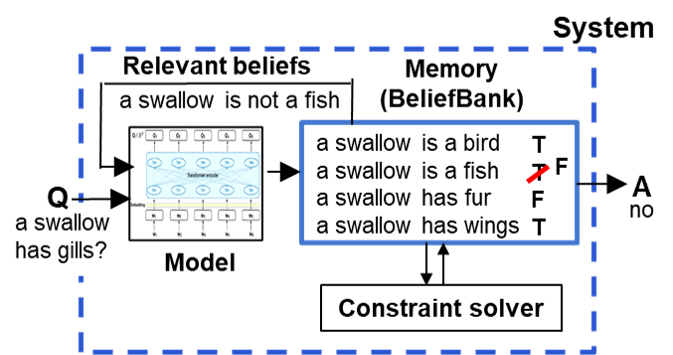
\includegraphics[width=1\columnwidth]{architecture3.png}	   % small figure
%      \vspace{-3mm}
\caption{ 
% \nk{As we do not consider exceptions I would use a different example. Maybe the swallow} 
The proposed architecture. The model's raw answers are stored in a
persistent memory (BeliefBank), and two mechanisms attempt to improve them:
(a) A {\bf constraint solver} flips beliefs that clash significantly with others
(b) A {\bf feedback} mechanism re-queries the model about those beliefs, but
uses other, relevant beliefs as the query context. We find both consistency and accuracy
of the overall system improves. \label{architecture}}
% \caption{The proposed architecture. A memory layer (the BeliefBank)
% plus constraint solver improves the consistency of beliefs.
% Given a new question, relevant beliefs are recalled to help improve
% the model's answers, thus feeding more accurate results back into the BeliefBank.
% \label{arcuitecture}}
 \vspace{-5mm}
\end{figure}

How might we ascribe a notion of belief to a model? Prior work has shown that, while
pretrained language models (PTLMs) contain substantial world knowledge \cite{Petroni2019LanguageMA, roberts-etal-2020-much},
their answers to probing questions can be inconsistent \cite{Elazar2021MeasuringAI, ravichander-etal-2020-systematicity, Kassner2020NegatedAM},
% models have high question-answering (QA) accuracy \nk{should we specify that we are talking about “closed-book question answering” and refer to papers that show that PLMs are good at it? }, they can also be inconsistent in their answers, 
making it hard to pin down what a model actually ``believes'' about a proposition.
% How might we ascribe a notion of belief to a model? Prior work has shown that, while
% models have high question-answering (QA) accuracy \nk{should we specify that we are talking about “closed-book question answering” % and refer to papers that show that PLMs are good at it? }, they can also be inconsistent in their
% answers, making it hard to pin down what a model actually ``believes'' about a proposition.
Our goal is to reduce this problem by having systems provide more globally consistent
answers to questions.

Prior work on reducing inconsistency has focused on retraining the model itself to be
more consistent in its answers, e.g., \cite{Ribeiro2019AreRR,Li2019ALF}, but with imperfect results. We present an
alternative approach in which the model is unchanged, but an evolving, persistent memory
of beliefs - called the BeliefBank - is layered on top, and two mechanisms use it 
to improve consistency among beliefs. First a reasoning component - a weighted SAT (satisfiability) solver -
flips beliefs that clash with others. Second, a feedback component re-queries the model
but using known beliefs as context, aiming for more accurate and consistent answers. 
Thus, the overall system attempts to build a more coherent representation of the
world from the model's raw answers, by ruminating on the answers seen so far.
This can also be viewed as assembling a simple ``mental model'' of the world \cite{JohnsonLaird1983MentalM} from
the noisy output of a raw PTLM.

\eat{
% I'm heartbroken to drop this paragraph!!!!! EMNLP perhaps?
In addition, 
just as the model helps populate the BeliefBank, we also show how beliefs in
the BeliefBank can improve the model's answers to future questions,
by using the most relevant beliefs as additional context for question-answering
(i.e., reminding the model of important facts pertinent to the new question).
These improved answers then feed into the growing BeliefBank, allowing the
overall system (model + BeliefBank) to continuously improve performance over
time, without retraining the model itself.
}

We explore this in a controlled experimental setting where 
both candidate facts and constraints are provided. Candidate facts are simple
sentences that may be true or false, e.g., "An eagle is a bird" (T), ``An eagle is a mammal'' (F). Constraints 
are between (variabilized) facts, e.g., ``X is a bird $\rightarrow$ X has wings''. These allow us both to probe and measure improvement
in the system's consistency and accuracy. % , described shortly.

\eat{
\red{Delete/reword this paragraph} Our approach involves an interplay between a model's raw answers, and an
evolving memory - the BeliefBank - of beliefs based on the model's earlier answers
and a set of constraints that should hold. Model's answers contribute to the BeliefBank,
and the BeliefBank contribute new context to help with future question-answering by
the model. In between, a constraint system serves to identify and reduce inconsistency
among beliefs in the BeliefBank. Combined, this results in a system capable of
continuous improvement over time, opening new possibilities for dialog and
interactive teaching.
}

We make the following contributions:
\begin{enu}
\item[1.] We augment a PTLM with a global memory - the BeliefBank -
and show how it can be leveraged to produce more globally consistent answers.
Specifically, we compare two mechanisms for using the BeliefBank - a reasoning and a feedback mechanism - 
and demonstrate that both can improve system accuracy and consistency in a restricted setting.
\item[2.] We contribute a controlled dataset to measure a PTLM's consistency against given constraints
\item[3.] We provide an analysis of the failure modes and directions for future work
\end{enu}
These are significant as they enrich a model's notion of ``belief'',
helping them construct a more coherent picture of the world. 

\eat{
PEC: Some of these are more activities (features) rather than contributions (benefits). e.g., Proposing
an architecture isn't a contribution per se - the contribution is showing a new architecture is beneficial.

We make the following contributions: i) We propose to augment a PTLM with a global memory - the BeliefBank to track a PTLM's "beliefs" ii) We compare two mechanisms of exploiting this BeliefBank - a reasoning and a feedback mechanism iii) We contribute a controlled dataset to measure a PTLM's consistency to given constraints. iv) We show that PLMs struggle with mutual exclusive constraints. v) Finally, we show that both mechanisms improve both overall accuracy and consistency on that dataset.
}

\section{Related work \label{related-work}}

% \nk{Some more related work- perhaps fold into the below: \cite{Talmor2020TeachingPM}, knowledge in PLMS 
% \cite{Petroni2019LanguageMA,roberts-etal-2020-much} \cite{kassner-etal-2020-pretrained}}
% \red{Possibly cite \cite{Graves2016HybridCU} - the memory there is more like
% an opaque expansion of the original network. I'm inclined not to cite this though
% as it's old and not really relevant.}

PTLMs are known to contain extensive world knowledge \cite{Petroni2019LanguageMA, roberts-etal-2020-much},
yet be inconsistent in their answers to probing questions \cite{ettinger-2020-bert,davison-etal-2019-commonsense, Kassner2020NegatedAM, ravichander-etal-2020-systematicity, Elazar2021MeasuringAI}.
While there has been some prior work on improving answer consistency, the primary approach
has been through modified model training. \citet{Ribeiro2019AreRR} improved consistency
by adding question paraphrases and question implications to the training data (data augmentation).
Others have trained models with (small) {\it sets} of examples with known constraints
between them, and included an additional loss term reflecting inconsistency among
set members during training \cite{Minervini2018AdversariallyRN,Li2019ALF,Asai2020LogicGuidedDA}.
However, the constraints are unused at test time (beyond what the model may have
internalized), and inconsistent answers are still produced.

For problems requiring a structured answer, e.g., predicting a sequence of
state changes, domain-specific constraints have been used to downgrade/block
answers that violate them \cite{Tandon2018ReasoningAA,Du2019BeCI}. This
encourages consistency within a single answer structure, but not among
different answers, our goal here.

% Concerning improving global consistency using constraints,
In the area of knowledge graph construction,
% , where individual extractions may be noisy, 
\citet{Pujara2013KnowledgeGI} define ``knowledge graph identification''
as the task of building a maximally consistent knowledge graph given noisy facts
and their extraction confidences, and ontological constraints between them.
They develop a solution use probabilistic soft logic (PSL) \cite{Broecheler2010ProbabilisticSL}
as their constraint reasoner. 
Similarly, \citet{berant2010global} learn the globally
optimal set of entailments between a large database of candidate
entailment pairs (with associated confidences), by applying
a global transitivity constraint (X$\vdash$Y \& Y$\vdash$Z $\rightarrow$ X$\vdash$Z)
using Integer Logic Programming. 
% Our constraint reasoner performs an 
% analogous task, but reasoning over noisy model predictions and domain-specific constraints.
In our case, we follow similar ideas but show how they can be usefully applied to the noisy predictions of a PTLM.
Specifically, we formulate the task as a weighted SAT (satisfiability) problem, and use 
the SMT solver Z3 \cite{z3} to solve it (Section~\ref{constraint-solving}).
% Our constraint solver (the SMT solver Z3 \cite{z3}) performs an analogous
% function, using the Z3 SMT solver (Section~\ref{constraint-solving}).
% \red{Say how we are different/go beyond.}

In the area of formal knowledge-bases (KBs), efficient algorithms
have been developed for detecting, measuring, and resolving inconsistency
\cite{hansen2000probabilistic,andersen2001easy,Thimm:2009d,muino2011measuring,Thimm:2013}.
Our contribution is to leverage some of these methods for PTLMs,
adding a reasoning capability that the PTLMs alone lack.

An important part of our contribution is the use of a dynamic, persistent memory.
While there are neural architectures that include an associated memory,
e.g., \cite{Henaff2017TrackingTW,Sukhbaatar2015EndToEndMN}, these components
typically play the role of a short-term working memory to help computation.
In contrast, our BeliefBank memory layer is a persistent, long-term memory of
explicit beliefs.

Finally, our feedback mechanism uses old answers to help answer new questions.
This builds on prior work such as Self-Talk \cite{selftalk},
where a model asks itself related questions to help with new answers.
In our case, feedback is selected from a global BeliefBank, rather
than generated with templated subqueries, potentially allowing more 
control over feedback selection.

\eat{
Finally, our feedback mechanism uses earlier answers to help with new questions.
This is closely related to, and builds on, prior work where a model uses
its own answers to subquestions as 

Finally, our feedback mechanism builds on prior work where answers to

builds on prior work where a model
asks itself appropriate subquestions, and uses those answers to help
answer a main question 
}
% \red{Mention self-talk and other self-feedback examples, \cite{shwartz-etal-2020-unsupervised}}

\eat{
% \subsection{PLMs and knowledge}
\subsection{Faithfulness}
\citet{subramanian-etal-2020-obtaining}
introduce the concept of module-wise faithfulness, a systematic evaluation of faithfulness in neural module networks for reasoning. We show that naive training does not produce faithful modules and propose several techniques to improve module-wise faithfulness. 
}
\eat{
\subsection{Inconsistencies in KGs}
(copied from old paper, need rewrite)
Consistency in KBs has been
studied in theoretical frameworks in the context of the
satisfiability problem and KB construction, and efficient
algorithms for detecting inconsistencies in KBs have been
proposed \cite{hansen2000probabilistic,andersen2001easy}.
Other work aims to quantify the degree to which KBs are
inconsistent and detects inconsistent statements
\cite{Thimm:2009d,muino2011measuring,Thimm:2013}.
% \cite{zhang2020need} showed that capturing factual knowledge inside PLMs is a specially resource hungry task.
}

\section{Task}

\subsection{Beliefs}

What does it mean to believe a proposition, say p = eagles are birds? In general, a system can
be said to (appear to) believe something if it acts as if it were true. In the specific
context of a QA system, we would expect it to produce answers consistent with p (and
its other beliefs). Pragmatically, we expect the system to (a) give a consistent answer to
different paraphrases of the question "p?" ("Are eagles birds?", "Is an eagle a type of bird?", ...),
and (b) give correct answers about implications of p ("Eagles lay eggs", "Eagles have feathers", ...).
% For example,
% if a system believes eagles are birds, and knows birds lay eggs (plus the rule of inheritance),
% we would expect it to answer "yes" to a question about whether eagles lay eggs.
Of course, a system may not perfectly answer such implications as the implications
may have exceptions, or the system may not be a perfect reasoner.\footnote{Similarly,
people do not always behave fully consistently with their professed beliefs.}.
Thus, to the external observer, there are {\it degrees} to which a system acts as if it
believes something.
% (Note this is distinct from a system's internal confidence in a belief).

\eat{
\red{Possibly delete this paragraph if too repetitive.} 
As has been shown elsewhere, language models (LM) can be inconsistent in their answers,
suggesting they have a rather weak notion of belief, in the sense described above.
To strengthen this, we add a dynamic memory component - the BeliefBank - on top of
the model to track and modify beliefs. We use the phrase ``the {\bf system}'' to refer
to the combined model plus belief bank. Our goal is to create a system with
a stronger notion of belief (i.e., more consistent and accurate) than the underlying LM inside it.
}

\subsection{Task Definition}

Our goal is to ascribe a stronger notion of ``belief'' to a system that includes a model $M$,
by improving the consistency and accuracy of its answers (compared with $M$). To measure
this we consider a true/false probing task, where we are also given a set of
constraints between answers:
\begin{myquote}
{\bf Given:}
\begin{ite}
\item a set of {\bf sentences} $S$ 
\item a set of {\bf constraints} $C(S)$ between (the truth values of) sentences in $S$, each annotated with a weight $w_i$ (A penalty $w_i$ is applied if $c_i \in C(S)$ is violated)
\item a {\bf model} $M$ that takes as input a True/False natural language (NL) question $Q$ and optionally an (NL) context $X$, and predicts a True/False answer $A$ with confidence score $F$
\end{ite}
{\bf Predict:}
\begin{ite}
\item the True/False labels for $S$, so as to maximally improve accuracy (with respect to gold labels) and
   consistency (minimize total penalties of constraint violations) compared with model $M$'s raw answers
\end{ite}
\end{myquote}
% As a toy example from Figure~\ref{example}, $S$ = \{penguin is a bird, penguin is a fish, penguin has fur, penguin has feathers, penguin has gills}, $C(S)$ = \{?X isa bird $\rightarrow$ NOT ?x isa fish, ?X isa fish $\rightarrow$ NOT ?x isa bird\},
% and the raw model $M$'s answers are \{T,T(wrong),F,T,T(wrong)\}. 
% \red{Move later} As our dataset class distribution (described shortly) is unbalanced, with significantly fewer True than False
% answers, we measure accuracy using F1 (over True questions) to avoid scores being dominated by negative
% answers.



\section{Approach}

% Our goal is to ascribe a stronger notion of ``belief'' to a model,
% by improving the consistency and accuracy of its answers. 
Our approach is to add a
memory layer, called the {\bf BeliefBank}, on top of the model to globally 
track beliefs. Two mechanisms are then used to modify BeliefBank beliefs, namely
(a) {\bf constraint reasoning} and (b) re-asking queries augmented with {\bf feedback} from the BeliefBank.

\subsection{Definitions \label{definitions}}

\eat{
\nk{Some comments on these definitions below: Can we find an alternative to $\textrm{tf}_i$? In our case the constraint is if X is True then Y is True/False. In general this could be also If X is False then Y is True/False. We could denote the belief as $\neg$ $s_i$/$s_i$ with an associated $w_i$ strength}

\red{Pete: I'm not quite comfortable with describing $s_i$ as an ``assertion''. An assertion is a statement
of fact or belief, but the $s_i$ themselves are just neutral sentences with no associated claims of truth or falsehood.
We could use the word ``statement'', if ``sentence'' sounds too syntactic (though as we've discussed,
the precise wording {\it is} important). Or perhaps each $s_i$ is (a sentence expressing) a statement about the world.?
Or each $s_i$ is (a sentence expressing) a possible assertion about the world?}

\red{Pete: Also, we do in fact reason with the truth values T/F of propositions, as illustrated in
Figures~\ref{architecture} and ~\ref{progression}, and in the SAT solver, so I wonder if we should call out the truth value as a 
separate entity. It seems a little strange to define $s_i \in S$ as a possible assertion, but then also say
$s_i$ is a belief. It shouldn't be both! I suppose we could say a belief is a (possibly negated) $s_i$ in the BeliefBank....}
}

\noindent Let
\vspace{-2mm}
\begin{ite}
  \item a {\bf belief} $b_i$ be a triple ($s_i$,$l_i$,$w_i$), where 
     \begin{ite}
     \item $s_i$ is a sentence $\in S$ % expressing a proposition about the world
      \item label $l_i \in$ \{T,F\} denotes the system's True/False belief about the truth of $s_i$
     \item weight $w_i$ is a number $\in [0,1]$ representing the system's strength of that belief
    \end{ite}
 For example:
 \begin{quote}
{\it      ("a poodle is a dog", T, 0.9) }
 \end{quote} 
 denotes the belief (strength 0.9) that "a poodle is a dog" is a true statement (T).
  \item a {\bf BeliefBank} $B(S)$ = a set of beliefs over assertions $S$ = $s_1,...,s_n$
%  \item For notational convenience, we denote the believed truth $l_i$ of $s_i$ according to $B(S)$ as $bel(s_i,B(S))$
 \item a {\bf constraint} $c_i$ = a 4-tuple of the form 
($s_i \rightarrow s_j, l_j, w_i$)
where 
\begin{ite}
\item $s_i,s_j$ are sentences $\in S$, 
\item $l_j \in$ \{T,F\} denotes the expected truth of $s_j$ if $s_i$ is true,
\item $w_i$ denotes the strength of that expectation (a penalty $w_i$ is applied if it is violated). 
\end{ite}
For convenience, we allow a shared variable X to be used in $s_i,s_j$, allowing a set of grounded
constraints to be expressed in a single statement, e.g.
\begin{myquote}
{\it (``X is a dog'' $\rightarrow$ ``X has a tail'', T, 0.8) }
\end{myquote}
expresses that if something is a dog, then it should (T) have a tail, with a penalty of 0.8 applied if
it does not. Mutual exclusivity is expressed using two rules, e.g., that fish and birds are mutually exclusive
is expressed:
\begin{myquote}
{\it (``X is a bird'' $\rightarrow$ ``X is a fish'', {\bf F}, 1.0) } \\
{\it (``X is a fish'' $\rightarrow$ ``X is a bird'', {\bf F}, 1.0) }
\end{myquote}
where ``F'' indicates the conclusion should be {\it false} if the condition is true.
% \nk{add mutual exclusive}
\item A {\bf constraint graph} $C(S)$ = a set of constraints $c_i$ over assertions $S$ 
% \red{This is problematic
% as $S$ in constraints (now) contain a variable ?X. So is $S$ sentences with or without variables?}
\end{ite}
Given a set of beliefs $B(S)$ about $S$ and a set of constraints $C(S)$, we measure
{\bf consistency} using (the complement of) \citet{Li2019ALF}'s conditional 
constraint violation ($\tau$) metric,
namely the fraction of constraints whose {\it condition} $s_i$ is believed true,
but whose {\it conclusion} (that $s_j$ has truth value $l_j$, denoted $l_j.s_j$) is not. 
In other words, over all constraints $c_i \in C(S)$, inconsistency $\tau$ is
\begin{myquote2}
$\tau = | \{ ~c_i~ |~ \neg (s_i \rightarrow l_j.s_j)~ \} | ~~~ / ~~~ | \{~ c_i ~|~ s_i ~\} |$ 
\vspace{1mm}
\end{myquote2} 
i.e., the size of the set of {\it violated} constraints ($s_i \rightarrow l_j.c_j$ is false)
divided by the size of the set of {\it applicable} constraints (i.e., those where the condition $s_i$ is true). We then define:
\begin{myquote2}
\begin{center}
consistency = 1 - $\tau$
\end{center}
\end{myquote2}

\begin{figure}[t]
\centering
     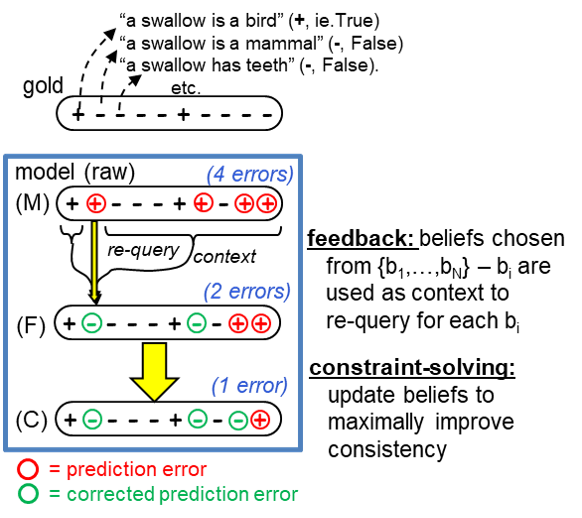
\includegraphics[width=1\columnwidth]{progression.png}	   % small figure
%      \vspace{-3mm}
\caption{Simplified illustration of iteratively improving the BeliefBank (oval). +/- denote true/false predictions for 10 facts about swallows. The model alone makes 4 prediction errors (M). Re-querying for those beliefs using other selected beliefs as context ({\bf feedback}) fixes 2 of those errors (F). Running {\bf constraint solving} on the updated BeliefBank fixes another error (C), resulting in just 1 error in the final BeliefBank. Here, the sequence is Model $\rightarrow$ Feedback $\rightarrow$ Constraints.\label{progression}}
% \caption{Simplified illustration of how the BeliefBank (oval) improves with time. +/- denote true/false predictions for 10 facts about swallows. The model alone makes 3 prediction errors (M). Alternatively, the model predicts batch1, making 1 error (A); using batch1 as context for batch2 results in only 1 new error (B); constraint solving fixes another error (C), resulting in just 1 error in the final BeliefBank (C).
% \label{progression}}
% \caption{Simplified illustration of how the BeliefBank (oval) improves with time. +/- denote true/false predictions for 10 facts about poodles. \nk{This example is a bit misleading. The raw answers are usually good with correct positive. A better example would be: a boa is a snake, a snake is a squamate, squamate is not a mammal, a boa is a mammal} The model alone makes 4 prediction errors (M). Alternatively, the model predicts batch1, making 2 errors (A); constraint solving fixes one (B); using batch1 as context for batch2 results in only 1 new error (C); constraint solving again fixes another error (D), resulting in just 1 error and greater consistency in the final BeliefBank (D). \label{progression}}
\end{figure}

\subsection{Methods}

We evaluate two methods for improving the BeliefBank's accuracy and consistency:
% using the constraints:
\begin{des}
\item[{\bf Constraint solving:}] Given a model $M$'s answers (with confidences) in the BeliefBank, a constraint
solver seeks to reduce constraint violations by potentially flipping answers that maximally clash
with other answers. 
% The answers in the revised BeliefBank are taken as the system's {\it overall} answers to questions.
\item[{\bf Feedback:}] Beliefs are checked by re-querying the model, but additionally
using relevant other beliefs as context for those (re-)queries. 
% Given a new question $q_{n}$, relevant beliefs in the BeliefBank are
% provided as additional input (namely as context) to help it answer $q_{n}$,
% to see if this improves the model's answer.
\end{des}
\vspace{1mm}
Figure~\ref{architecture} shows these components, and 
Figure~\ref{progression} illustrates how they can iteratively improve the BeliefBank.
In Figure~\ref{progression}, there are 10 beliefs of interest about swallows. When probed about these, the raw model 
gets 4 of these wrong, including inconsistently believing that a swallow is both a bird and a mammal
(see (M) in Figure~\ref{progression}). Applying feedback, we re-ask the model the 10 questions but adding 
in the most relevant known beliefs as context for those (re-)queries. The BeliefBank is updated with
these new answers, fixing 2 of the errors (F). We then run the constraint solver over the BeliefBank,
resulting in one answer being flipped (question 9, from T to F), thus fixing another error (see (C)). 
The final BeliefBank has just 1 error and greater consistency.  
% As we describe later, we also evaluate applying update (e.g., first constraint-solving then feedback) to identify which is most effective. 
Note that updates can also 
introduce new errors (not shown in Figure~\ref{progression}), so improvement is not guaranteed. 

\subsubsection{Constraint Solving \label{constraint-solving}}

Given a set of beliefs and constraints, the constraint solver has two competing objectives: (a) flip 
beliefs so as to minimize constraint violations (b) don't flip beliefs, so as to preserve
the model's raw beliefs, i.e., minimize conflict between the model and BeliefBank. 
To implement this tradeoff, the model's beliefs are themselves treated as just
another constraint, e.g., the belief "a poodle is a dog" (weight 0.9) is treated as a constraint
"a poodle is a dog", with penalty 0.9 if it is violated (i.e., labeled as false by the constraint solver).
To balance the two objectives (a) and (b), the belief weights are scaled by a learned hyper-parameter $\lambda$,
trained on a calibration part our dataset, disjoint from the data then used in experiments (Section~\ref{dataset}).

To implement constraint solving, we translate the task into a {\it weighted SAT} (satisfiability) problem $P$,
for which efficient algorithms with guarantees exist. Each belief becomes a weighted assertion in $P$, e.g.,
the belief ("a poodle is a dog", T, 0.9) is expressed in SAT syntax:
\begin{myquote2}
{\it 0.9 } % \footnote{In practice, as Z3 SAT syntax requires integer weights, we multiply all weights by 100 then drop decimals.}
{\it "a poodle is a dog"}\footnote{In practice, strings are replaced with numeric identifiers in SAT syntax, but for clarity we leave them as strings here.}
\end{myquote2}
while the constraint ("a poodle is a dog" $\rightarrow$ "a poodle has a tail", T, 0.8) is expressed:
\begin{myquote2}
{\it 0.8 "a poodle has a tail"   ~{\bf -}"a poodle is a dog"}
\end{myquote2}
(literally: {\it "a poodle has a tail"} OR NOT ("{\bf -}") {\it "a poodle is a dog"}). 
We then apply the solver Z3 \cite{z3} to $P$, which outputs a set of truth assignments for all individual 
sentences in $P$ so as to minimize the weighted sum of violations. If the truth assignment of any sentence
has changed, the BeliefBank is correspondingly updated. % \red{How do we update the weights?}.

% To find the optimal solution to the constraint equations, we convert the problem into a weighted SAT problem,
% and then use the Z3 SAT solver to find the optimal truth assignments to the beliefs. \red{Details are in
% Appendix~\ref{??}}.

\subsubsection{Feedback}

Feedback involves re-asking the model a question, but with the benefit
of knowing answers to related questions. To use these answers in the re-query,
selected beliefs are added to the query context before re-asking the model.
(Note that the selected beliefs are not guaranteed to be correct, of course).
Our conjecture is that if the model is explicitly reminded of relevant beliefs when answering a new question,
it will answer the question more accurately and consistently.
For example, in Figure~\ref{architecture}, when asked "Do swallows have gills?", our model $M$ incorrectly answers "yes".
But if reminded that swallows are not fish, by asking: "CONTEXT Swallows are not fish. QUERY Do swallows have gills?" 
the model now correctly answers "no". 

We evaluate two policies for choosing which beliefs to feed back to $M$ when re-asking question $Q$:
\begin{enu}
\item[1.] randomly selected from the BeliefBank
\item[2.] most relevant, using the constraint graph to identify relevance. As the constraint graph captures potential clashes that the answer to  $Q$ could cause, we use the graph to select those beliefs that would be most affected by that answer. % (according to the raw constraint penalties). 
For example, if the current query is: "Is a poodle an animal?", the constraint graph identifies potential clashes the would occur if the model
answered "yes", and also clashes if it answered "no". In this example, if the model answered "no", the resulting belief ("a poodle is {\it not} an animal") would strongly clash with other beliefs "A poodle is a dog.", "A poodle is a mammal.", and "A poodle is a domesticated canine.", so all three are strong candidates for the context. We select the three overall strongest clashing beliefs found in this way, considering both a "yes" and a "no" answer to $Q$.
% item[2.] most relevant, using the constraint graph to identify relevance: The constraint graph captures the potential clashes the answer to the current query could induce. The beliefs which are strongest effect by the answer to the current query (according to the raw constraint penalties) are selected as context: If the current query of interest is: "Is a poodle an animal?" the constraint graph identifies potential clashes in case the model answers "yes" or "no". If the model's answer would be "no" it would strongly clash with ("A poodle is a dog.", "A poodle is a mammal.", "A poodle is a domesticated canine."), therefore these are selected as context.
\end{enu}
In both cases, three (if possible) beliefs are selected, this number empirically found to be most effective. (For experiments with small amounts of data, sometimes less than three relevant beliefs are found.)

\section{Dataset \label{dataset}}

% \red{Still to do a pass over}

We create a dataset to test our approach in a controlled way, allowing us to perform systematic experiments to evaluate behavior.
The dataset contains two parts, {\it constraints} and {\it facts}, defined over simple sentences
such as ``a swallow is a bird.''.

\subsection{Constraints}

The dataset contains two kinds of constraints:
\begin{des}
\item[{\bf positive implications:}] (conclusion truth value $\textrm{l}_i$ = True), e.g.,
\begin{myquote}
{\it ``X is a dog $\rightarrow$ [TRUE] X has a tail.''}
\end{myquote}
\item[{\bf mutual exclusivities:}] expressed as a pair of constraints with $\textrm{l}_i$ = False, e.g.,
\begin{myquote}
{\it ``X is a dog $\rightarrow$ [$\textrm{l}$=FALSE] X is a bird.''} \\
{\it ``X is a bird $\rightarrow$ [$\textrm{l}$=FALSE] X is a dog.''}
\end{myquote}
expresses that an entity cannot be both a dog and a bird at the same time.
% These are expressed as a pair of constraint templates each with $\textrm{tf}_i$ = False:

\end{des}
Positive implications were manually gathered from ConceptNet \cite{Speer2017ConceptNet5A}.
First, we identified 176 general concepts of interest, e.g., ``mammal'', choosing concepts
with high occurrence ($>$ 100 times) in ConceptNet, avoiding significantly ambiguous terms (e.g., ``bat''), and filtering out plurals and 
obscure concepts.
% irrelevant concepts. \nk{was not sure how to call "general non-sense or uninteresting things"}.
For these entities, we then collected all ConceptNet facts involving 6 relations: IsA, HasA, MadeOf, PartOf,
HasProperty, and CapableOf, and
% \red{[]generate all possible transitive implications - PEC: Not sure what you mean...]}
re-expressed them as constraints. For example, the ConceptNet triple (dog, HasA, tail) gives rise to the constraint
"X is a dog" $\rightarrow$ "X has a tail." % (X, IsA, dog)$\rightarrow$ (X, HasA, tail). 
(Triples are converted into English sentences using simple templates).
We then manually filter theses constraints for factual correctness.
We also add the constraint in the backwards direction, "X has a tail" $\rightarrow$ "X is a dog",
expecting these to have lower weight, i.e., be weaker.
(These backwards rules discourage the trivial solution that everything is false.)
Finally, weights are assigned to
all the constraints using a combination of crowdsourcing and calibration,
described shortly (Section~\ref{section:penalties}).
% , and also consider the constraint in the reverse direction "X has 
% We also add the constraint in the reverse direction, assigning a weaker weight as described shortly

\eat{
resulting in 
to exclude wrong implications like \red{XXX}. Finally, we use crowdsourceing to validate these constraints, see \ref{section:penalties}.
}
\eat{Mutual exclusivities were gathered from a filtered subset of the WordNet taxonomy,
based on the approximation that (generally) siblings in the WordNet noun hierarchy
are mutually exclusive \red{elaborate}.
}

Mutual exclusivities were gathered from the ``isa'' taxonomies in ConceptNet and WordNet \cite{wordnet},
using the approximation that (generally) siblings in the noun hierarchy are mutually exclusive.
Thus, for any pair of concepts in our concepts of interest that reside in different taxonomic subtrees,
we add a mutual exclusivity constraint (using two constraint rules). 

We collected 12,147 constraints in this fashion (1798 implications, 8599 mutual
exclusivities). The set of constraints can be % usefully
viewed as a {\it constraint graph} of implications from one sentence to another.

\subsection{Constraint Weights}
\label{section:penalties}
We used a combination of crowdsourcing and calibration to assign a reasonable
constraint weight $w_i$ to each constraint. Workers were shown each
constraint and asked to judge if the implication held always/usually/sometimes/rarely/never with raw scores 
4/3/2/1/0. 
% The below not relevant here:
% This scoring procedure is used for forward implications as well as in the backwards direction. Backwards evidence is needed to prevent the SAT solver from flipping all answers to "no" which would result in perfect consistency but low accuracy. Rather than an actual implication, the backwards direction is evidence for a sentence to be true, e.g., "X has feathers.", "X has wings." and "X has two legs." accumulates to strong evidence for "X is bird." 
Three workers independently scored each constraint and the scores averaged.

When used with a particular model $M$, the raw scores need to be recalibrated
to appropriately match the confidences output by that model. This is described shortly in Section~\ref{calibration}.

\subsection{Facts}

We also collect a set of truth-labeled facts about different entities, relevant to the constraints.
To do this, we select a new entity, e.g., "poodle", that is a member of one of our general concepts,
e.g., "dog", then instantiate the constraint graph with that
entity (i.e., set X = "poodle"). We then identify the leaf (source) nodes of that graph, just considering
forward implication rules, i.e., find facts not implied by other facts in the graph, and manually
annotate their True/False labels. We then use the implications to infer
other True/False labels for other sentences, i.e., propagate the annotated labels through the graph.
This provides ``silver'' labels for sentences reachable in this way (a subset of all the sentences 
in the graph), silver because the implications are soft, hence not guaranteed to hold for all entities. 

We repeat this for 27 entities (17 animals, 10 plants), resulting
a final dataset containing 4998 ``silver'' facts (sentences + True/False labels).
\eat{Note that each slice is independent and can be processed separately.
As described shortly, we perform our experiments with each slice in turn
and average results.}


\eat{
\subsection{Query and sentence templates}
\nk{Not sure where to put this section}
In order to query the model for its belief we manually define template queries for each relation, e.g., for the IsA relation the template query "Is X a Y?" is used.
These template queries are then instantiated for each sentence of the constraint set by filling in the relevant objects Y, e.g., "Is X a dog?".

We then query the model's beliefs involving an entities of the test set by filling in the subject slot X, e.g., "Is a poodle a dog?".

We also define an additional set of sentence templates, e.g., "X is Y." which are used to feed back beliefs into the context window of the model.
}


\eat{\subsection{Templates}

We collect all the unique variabilized sentences in the constraints together,
resulting in 200 \red{??} sentence templates, e.g., ``?X is a dog.''.
}

\begin{table*}
\centering
{\small
\begin{tabular}{|l|ll|ll|ll|} \hline
Results after seeing \% of data $\rightarrow$ & \multicolumn{2}{|c|}{\bf 10\%} &
\multicolumn{2}{|c|}{\bf 50\%} &
\multicolumn{2}{|c|}{\bf 100\%} \\
Accuracy (F1), Consistency (1-$\tau$) $\rightarrow$ & F1 & Con & F1 & Con & F1 & Con\\ \hline           
model (raw) & 75.07 & 87.06 & 74.29 & 77.11 & 73.25 & 74.68 \\
\eat{model + constraint-solving & 80.2 & 100.0& 88.72 & 99.81 & 88.42 & 99.60 \\}
model + constraint-solving & 81.23 & 100.0 & 89.80 & 99.93 & 91.90 & 99.83 \\
model + feedback (random)& 85.33 & 93.46 & 84.59 & 87.59 & 84.00 &88.02  \\
%model + feedback (random positive)&  & &   &  &  &  \\
model + feedback (using constraints)& 82.04 & 94.69 &84.74&92.24&88.28&91.00 \\
%model + feedback (most confident)\\
model + feedback (using constraints) + constraint-solving & 83.69 & 100.0& 91.66 & 99.53 & 93.40 & 99.42\\ \hline
%model + constraints + feedback (relevant for query + flipped)&&&87&90 & & \\\hline
% model + feedback (random positive) &&&&\\
% model + feedback (most confident) + constraints &&&& \\\hline
\end{tabular}
}
\caption{Results after seeing different proportions of data.
{\bf model (raw)} are scores for the model stand-alone.
In {\bf model + constraint-solving}, the constraint solver is run over all
the raw answers so far. In {\bf model + feedback}, questions are re-asked
using context selected from the other raw answers so far. In {\bf model + feedback + constraint-solving},
the constraint solver is additionally run on the answers with feedback. 
\label{results}}
\end{table*}


\section{Experiment Environment}

\subsection{Model}

The fixed model $M$ that we use for our experiments is the multi-angle QA system MAQAw \cite{arc-da}.
MAQAw is a derivative of UnifiedQA, a state-of-the-art T5 model fine-tuned on $\approx$400k question-answer pairs
\cite{unifiedqa}. MAQAw was then 
further fine-tuned on several thousand science questions and trained on different permutations of inputs and outputs
(e.g., query Q + context X $\rightarrow$ answer A; XA $\rightarrow$ Q; etc.). 
To query the model's beliefs we pose the query and let the model chose between the two answer options "yes" and "no".
MAQAw also outputs an answer confidence, used as the belief weight. Note that we do not retrain MAQAw for
this work; rather, it is used as a black-box QA module in the broader system (Figure~\ref{architecture}).
%NOTE this model is fixed for our experiments here.



\subsection{Calibration \label{calibration}}

To appropriately mix MAQAw's confidences and the constraint scores, a calibration step is needed. To do this,
we use the 1239 facts about seven entities in our dataset as a calibration set, and then perform
experiments using (only) the remaining facts. 

We calibrate the crowdsourced raw constraint scores using sigmoid-scaling (two parameters).
We also calibrate the relative weight $\lambda$ of the model's beliefs and the constraints,
the relative weight of the backward implications (compared with the forward), and 
the relative weight of mutual exclusivity rules.
To do this we perform a grid search over these parameters, finding the values that result in
the highest F1 (accuracy) after running the constraint solver over the raw model's beliefs about
these facts.

\eat{
Using the calibration facts, we perform a grid search 
\subsection{Calibration}
For constraint solving constraint and belief
weights have to be well calibrated. We use a small set of seven entities and their grounded test set for calibration and maximize F1.

The crowdsourced raw constraint scores were calibrated by sigmoid-scaling, using a
grid search over slope and shift to identify the scaling hyper-parameters. We also calibrate the relative weight of the model's beliefs and the constraints, and the relative weight of the forward, backwards and mututal exclusivities. \nk{Should I put more details in the Appendix?}
}

\eat{
\begin{table*}
\centering
{\small
\begin{tabular}{|l|ll|ll|ll|} \hline
Accuracy (F1), Consistency $\rightarrow$ & F1 & Con \\ \hline           
model (raw) & 73.25 & 74.68 \\
model + SAT (model constraints) &  &\\
model + SAT (additional human intervention) &  \\\hline
%model + constraints + feedback (relevant for query + flipped)&&&87&90 & & \\\hline
% model + feedback (random positive) &&&&\\
% model + feedback (most confident) + constraints &&&& \\\hline
\end{tabular}
}
\caption{Constrains captured by model vs. human intervention
\label{results_human_intervention}}
\end{table*}
}

\eat{
\begin{table*}
\centering
{\small
\begin{tabular}{|l|ll|ll|} \hline
Results after seeing $\rightarrow$ & \multicolumn{2}{|c|}{\bf batch1} &
\multicolumn{2}{|c|}{{\bf batch2}} \\
Accuracy (F1), Consistency $\rightarrow$ & F1 & Con & F1 & Con\\ \hline           
model (raw) & 74 & 77 &74 & 75 \\
model + SAT & 89&100& 88&100\\
model + feedback (random)& - & - & 85 & 89\\

model + feedback (relevant for query constraints)&-&-&88&91\\\hline
%model + constraints + feedback (relevant for query + flipped)&&&87&90\\\hline
model + feedback (random positive) &&\\
model + constraints + feedback (most confident) &&\\\hline
\end{tabular}
}
\caption{(old table)}
\end{table*}

\eat{\begin{table*}
\centering
{\small
\begin{tabular}{|l|ll|ll|ll|ll|} \hline
Results after seeing $\rightarrow$ & \multicolumn{2}{|c|}{\bf batch1} &
\multicolumn{2}{|c|}{+ {\bf batch2}} &
\multicolumn{2}{|c|}{+ {\bf batch3}} &
\multicolumn{2}{|c|}{+ {\bf batch4} (all)} \\
Accuracy (F1), Consistency $\rightarrow$ & F1 & Con & F1 & Con & F1 & Con & F1 & Con \\ \hline           
model (raw) & 48 & 76 & 28 & 79 & 42 & 75 & 44 & 72\\
model + constraints & & & & & & & & \\
model + feedback (bm25) & 48 & 76 & 39 & 92 & 48 & 78 & 58 & 86\\
model + feedback (random) & 48 & 76 & 42 & 94 & 56 & 86 & 56 & 81\\
model + constraints + feedback (most confident) & & & & & & & & \\
model + constraints + feedback (relevant for query) & & & & & & & & \\
model + constraints + feedback (relevant for query + flipped) & & & & & & & & \\\hline
\end{tabular}
}
\caption{{\bf model (raw)} shows the accuracy (F1) and consistency (Con) of the
model stand-alone, after each batch of questions. 
 In {\bf model + constraints}, the constraint solver is run
 after each batch on all the answers seen so far. In {\bf model + feedback},
 questions in batch2 are posed to the model along with selected beliefs from
 all earlier batches (batch1), but the constraint solver is unused. 
 {\bf model + constraints + feedback} is the same, except the constraint solver is also run
 after each batch on all answers seen so far.
\label{incremental-improvement}}
\end{table*}
}
}

\section{Experiments}

We evaluate accuracy (F1)\footnote{
We measure accuracy with F1 (on the True class) rather than \% correct because
the True/False distribution in our dataset is unbalanced, with significantly fewer True than False
answers. F1 avoids scores being dominated by negative answers.}
and consistency (1-$\tau$, Section~\ref{definitions}) 
for 3 different-sized, randomly selected subsets of our data: 10\%, 50\%, 100\%. We average results across entities.
The results are shown in Table~\ref{results},
showing the model's a priori accuracy and consistency (line 1),
and the effects of constraint-solving, feedback, or both (lines 2-5).

\subsection{Results}

\noindent
Several conclusions can be drawn: % from these results:
\begin{enumerate}
\item {\bf The basic model is both imprecise and inconsistent,} with F1 $\approx$ 73\% and consistency $\approx$ 75\%.
This reflects similar observations of model inconsistency made for other PTLMs (Section~\ref{related-work}), and illustrates the
challenge we wish to address. As we show shortly, the main source of error is in precision, rather than recall,
i.e., the large majority of errors are false positives.

%\noindent
\item {\bf Constraint-solving removes almost all inconsistency} with respect to our constraints, even with
only a subset of the data. (Of course, with less data, there are fewer applicable constraints that can be
violated.) It also {\bf significantly improves accuracy} ($\approx$+10\% F1), indicating
that the flipped truth values not only reduce clashes but better align with the true (gold) labels. Note
that improvement in accuracy is not guaranteed: constraint-solving can (and sometimes does) flip
truth values the wrong way, in order to reduce constraint violations. The improvement suggests 
that the model is getting enough answers correct, a priori, to steer the constraint-solving in
the right direction. Comparing accuracy after seeing 10\%, 50\% and 100\% of the data, we note incremental gains the more beliefs and constraints the constraint-solver is able to leverage.   

%\noindent
\item {\bf Feedback (both types) also improves both accuracy and consistency}, although not
to the same extent as constraint-solving. It is perhaps surprising that explicitly reminding the model
of facts it already believes, when answering a new question, can improve the results.
The context may be behaving loosely like an attention mechanism, encouraging the
model to focus on the facts provided in the context, even if they are already latently known,
thus influencing question-answering behavior. Similar observations have been observed by \citet{selftalk}. 

%\noindent
\item {\bf Constraint-guided feedback is more effective than random feedback} when the BeliefBank is
large (100\% column), with F1 rising to 88\% and consistency to 91\%. 
% As for the constraint-solver, constraint-guided feedback needs more data to be effective. 
Conversely, % \eat{it is surprising that gains are less with lower amounts of data (e.g., 10\% column), where} 
randomly selected feedback perform similarly across different data sizes. We analyze this further in Section~\ref{analysis}.

%\noindent
\item {\bf Combining constraint-guided feedback with constraint solving further improves accuracy} by $\approx$5 percent points compared with only using feedback,
and by $\approx$2 percent points compared with the constraint-solver alone.
Again the addition of the constraint-solver results in
almost perfect consistency of 99\%. This setup reflects the incremental setup depicted in Figure \ref{progression}, where 
the constraint-solver can leverage the updated BeliefBank.

\end{enumerate}

\subsection{Analysis \label{analysis}}

Both constraint-solving and feedback can cause the overall system to flip beliefs, with
the goal that the overall system's beliefs (in the BeliefBank) are more accurate and consistent
than those of the underlying model. However, both mechanisms have the potential to flip
beliefs in the wrong direction also. We provide some analysis of both good and bad flips
here.

\paragraph{The System Behaving as Desired:} 
As an illustration of desired behavior, the raw model incorrectly believes that a pine is both a plant (correct) and a
vertebrate (incorrect), when queried. However, this violates a mutual exclusivity rule, so the constraint-solver
considers flipping one of these. Flipping ``pine is a plant'' from T to F would result in 
numerous other violations, e.g., ``pine is a tree'' (which the model also believes)
would become violated. As a result, it prefers to (correctly) disbelieve ``pine is a vertebrate'', improving
both the accuracy and consistency of the BeliefBank.

\paragraph{Types of Error:} From an analysis of the data, we see that the majority of the raw model errors
are false positives - the MAQAw model generally answers (almost) all the positive facts correctly (recall is $\approx$97\%),
but mistakenly thinks some negative facts are also true (precision is $\approx$60\%).
These false positives are typically rather unusual facts, e.g., ``A poodle is a bathroom.'' (MAQAw's answer: True).  
It is unsurprising that the model knows most of the positive facts, as they are simple statements about 
common entities (``eagles can fly''), likely seen in pre-training. However, the fact that the model 
makes (what a person would view as) catastrophic errors when asked more unusual
questions, e.g., believing that ``a poodle is made of fermented milk and bacteria'', 
reveals that the PTLM's grasp of the world is still incomplete and problematic. The constraint mechanism
proposed here essentially asks the model to think about its answers and their consequences,
so that it can spot problems that the PTLM alone does not see, and repair them accordingly.

\paragraph{Sensitivity to Constraints and Weights:} 
The constraint reasoner also makes mistakes, sometimes flipping things the wrong way
so as to improve consistency, at the expense of accuracy. For example, the raw model
correctly believes that a ``a rat is not a cat''. 
However, the constraint solver then (incorrectly) flips this to "a rat is a cat". It does this as
% Due to misleading constraints the constraint-solver flips to ``a rat is a cat''. It does this as
there are multiple constraint rules weakly suggesting rats are cats given the model's other beliefs
% as the model correctly and incorrectly believes ``rats
(''rats catch mice'', ``rats have tails'', ``rats have fur'',...), which together add up. However,
the model {\it also} (correctly) believes ``a rat is not a feline'', and there is a constraint
that ``a cat is a feline'', so in principle this should prevent the belief ``a rat is a cat''.
In practice, though, the constraint ``a cat is a feline" does not have infinite weight,
so here the constraint mechanism allows it to be violated, allowing the wrong
conclusion (``a rat is a cat'') to be drawn.

Of course, one could increase the weight on the ``a cat is a feline'' constraint
to solve this particular problem, or add new constraint rules like ``cats are larger than squirrels''. In general, though,
the effectiveness of constraint reasoning is sensitive to both the number
and weights on the constraints. Although we have used automated techniques
to re-calibrate the various weights (Section~\ref{calibration}), the system's
behavior remains sensitive to them. Finding more effective ways to discover and
appropriately tune constraints remains an open problem.

\paragraph{Ambiguity:} Although we have avoided obvious cases of ambiguity, e.g., reasoning
about ``bats'', there are smaller cases of ambiguity that may explain some of the raw
model's errors. For example, although the model (incorrectly) believes "a swallow is a fish",
there {\it is} a fish called "a black swallower" that it may have seen in pre-training,
confusing it. Similarly, some unusual statements such as ``A penguin is a protein''
(gold label is False, model believes is True) are partially ambiguous, possibly
contributing to the discrepancy.

\paragraph{Does the Model Know the Constraints?} 
Finally, we are checking consistency using {\it externally} defined constraints,
which the raw model may not itself be aware of (i.e., may not have acquired in pre-training). 
For example, although the model may {\it appear} to be internally inconsistent if it thinks a swallow is both a bird 
and a fish, this is only true if it also knows these beliefs are mutually exclusive.
To check for {\it internal} inconsistency of a model's behaviour, we would also need to
check if the model knew the violated constraints themselves, e.g., using additional probes.
Again this is an area for future exploration.

\paragraph{The influence of Feedback:} We currently can only speculate why feedback (i.e., providing relevant
facts to the model as context for question-answering) improves results. One explanation is that
feedback helps the model focus attention. For example, reminding the model that "a swallow is not
a fish" should help it realize that "a swallow has gills" is False (Figure~\ref{architecture}).
However, we also observe significant gains when feeding back random facts about the entity
being queried. Possibly these facts still encourage the model to focus on the entity. Or,
given the majority of beliefs are negative, the simple presence of negation in the context
may discourage false positive answers, the primary cause of raw model errors.

\eat{
We present the results of three sets of experiments in this environment:

\begin{enu}
\item[\textbf{1. Model:}] How accurate and consistent is the model, a priori?
\item[{\bf 2. Model + Constraint-solving}] To what extent does adding a BeliefBank memory layer and a constraint solver improve the consistency and accuracy
           of the overall system (model + BeliefBank)?
\item[{\bf 3. Model + Feedback:}] To what extent does a feedback mechanism based on the BeliefBank memory layer improve the consistency and accuracy?
\end{enu}

% Given a set of questions $q1,...,q_n$ about sentences $S$, we can pose them to $M$ and collect both the answers (True/False)
% and confidences to form the raw model's beliefs $B_{model}(S)$ about $S$.

\subsection{Model}

How accurate and consistent is the model, a priori?

Results show models aren't perfectly consistent in their beliefs. Especially mutual exclusivities are not well captured by the model, e.g. "A swallow is a bird" and "A swallow is a mammal." The missing understanding for mutual exclusivities can result in quite obscure beliefs, e.g., "A poodle is a bathroom.". One could argue that is is not fair to ask a model these kind of questions as it has not seen similar data during training. One the other hand, humans are also able to generalize mutual exclusivities easily. When aiming for human-like intelligence this kind of generalization without the need to see these facts explicitly is necessary. Generally, the model has a high 
recall (97.38) and low precision (59.61). 

\eat{We also evaluate the amount of constraints the model captures internally. To do so, we reformulate the constraints into a single query: "X is bird." $\rightarrow$ "X has wings." is queried directly by "Does A bird have wings?". We use multiple paraphrases of the query and provide the answer options: (A) always (B) mostly (C) sometimes (D) rarely (E) never. Each answer option is 'never': -1, 'always': 1, 'rarely': -0.5, 'sometimes': 0.0, 'mostly': 0.5, "yes": 1.0, "no": -1.0. only half of the mutual exclusive constraint are captured by the model but all of the positive implications. Therefor, . Just using the model's constraint is a . The missing . 
We aggregate predictions scores acorss the paraphrases}

\subsection{Model + Constraint-solving}

% The model alone is inconsistent in its beliefs, making it hard to identify what its ``opinion'' is.

We now attempt to do better, by adding a memory (a BeliefBank) plus a reflective component (a constraint solver)
to the overall system. By ruminating on the model's raw beliefs, the constraint solver may determine
that some beliefs should be flipped based on the weight of evidence from other beliefs. \eat{We refer
to the combination of the model plus memory (BeliefBank) as ``the system'', whose beliefs are those
in the maintained BeliefBank.}

Results show that the constraint solver improves both the consistency and correctness
of the system's beliefs.

The constraint solver gives control over and interpretable results but relays on a careful calibration and the right constraints being in place.
Missing constraint or overestimated weights can enforce wrong flips. Overall, the SAT solver is good in extracting the core beliefs about an entity, e.g., "A poodle is a dog". \nk{Need a clear definition how we define core beliefs}

Most of the flips are resolving mutual exclusivity clashes. 

\nk{mention wrong flips: boa is a snake and a cat}

% \begin{figure}[t]
%\centering
%     \includegraphics[width=1\columnwidth]{architecture.png}	   % small figure
%\caption{The model's raw answers are stored in a persistent memory (BeliefBank),
%and potentially flipped if they clash significantly with others. Pertinent
%beliefs are then used to help the model answer new questions. We find both
%consistency and accuracy of the overall system improves. \label{architecture}.}
% \vspace{-3mm}
%\end{figure}

\subsection{Model + Feedback}

Can we use the beliefs in the BeliefBank to improve answers to {\it new} questions by the model?
To do this, given a new question, relevant beliefs are used as 
context to the model for question-answering, as illustrated in Figure~\ref{architecture}. 
By reminding the model of corrected or salient beliefs, we conjecture that the model itself
will improve its question-answering ability, in turn potentially improving the
BeliefBank.

We evaluate two policies for selecting relevant beliefs for a new question:
\begin{des}

\item[(a)] The top 3 {\it most relevant beliefs} according to the constraint graph. 
%\item[(b)] The top r {\it most confident beliefs}.
\item[(c)] 3 {\it randomly chosen beliefs}
%\item[(d)] 3 {\it randomly chosen positive beliefs}
\end{des}

We find that providing the model the ability to consult with it's prior belief generally helps to improve accuracy and consistency. Surprisingly, also randomly selecting prior belief and adding them to the context window helps substantially. This seems to be due negation markers in the context window inducing more tendency to answer "no". Using the constraint graph to select relevant beliefs instead of random ones results in both higher accuracy and consistency. 

Generally, consistency improvements using the context window are lower than the combination of model and SAT solver. In comparison to the SAT solver the results are less interpretable.
% Given the new answer, we run the constraint solver as usual. We are interested in whether
% an improved model (using one of these policies) + constraint solver will outperform a fixed
%  model + constraint solver.
}
\eat{To evaluate performance on a new, unseen questions,
we divide the dataset randomly into two batches.
% , and incrementally provide each
% batch to the overall system (rather than evaluate incrementally for every instance).
First the model answers all questions in $batch_1$ with no context, and the BeliefBank
is created. Then, the model answers all
questions in $batch_2$ with a context provided from the BeliefBank ($batch_1$) questions,
and the constraint solver rerun. We similarly repeat for $batch_3$ and $batch_4$.
Results are shown in Table~\ref{incremental-improvement}.
}

\section{Future Work}

% This work is a first step towards endowing PTLMs with a globally consistent notion of beliefs. By augmenting a PTLM with an additional global 
% memory and reasoning component - the BeliefBank - we showed that both accuracy and consistency can improved. 

These findings were made using a restricted experimental setup where facts are short sentences, constraints are provided, and both facts and constraints use the same language so it is clear when constraints apply. To broaden the approach, several developments are required:
\begin{ite}
\item
A system would need to {\bf automatically gather constraints and queries}.
Constraints might be mined from text, or even extracted from the model itself by direct querying. Alternatively, domain-specific constraints (e.g., ``X is a bird $\rightarrow$ X has wings'') could be replaced with more generally applicable constraint patterns
(e.g., ``X is a Y \& Y has Z $\rightarrow$ X has Z''), turning the domain-specific parts of constraints into facts that
themselves could reside in the BeliefBank.
\item Our queries have been simple facts. To fully utilize the BeliefBank for more complex
queries (e.g., ``What color is the gas that plants produce?''), a mechanism would be needed to {\bf decompose compound queries
into their primitives} (``What gas do plants produce?'', ``What color is that gas?''), and ensure they were
consistent with BeliefBank beliefs (e.g., ``Oxygen is colorless''); in other words, ensure complex answers were {\it faithful} 
to the BeliefBank \cite{Subramanian2020ObtainingFI}.
\item In general, detecting when a constraint applies to a fact is non-trivial, and requires appropriate machinery for
{\bf identifying sentence/constraint alignment}, e.g., an entailment model \cite{Seo2017BidirectionalAF}.
\item Although constraint/model weights are automatically calibrated (Section~\ref{calibration}), the
system is still sensitive to those weights and can make mistakes (Section~\ref{analysis}). {\bf Improved mechanisms for automatic calibration}
would significantly help.
\item Our system is passive, in that it answers questions and uses answers in the order they are provided. An alternative design
would be an {\bf active system} that, given a new question, actively identifies which auxiliary questions would be most
useful to also ask, to help answer the main question (either with constraint solving or feedback).
\end{ite}
Finally, scaling to a massive BeliefBank would require addressing several engineering requirements,
including bounding the constraint checking, and not re-asking every prior question as new answers were discovered.
For example, we might only check constraints
and their implications up to depth $D$ from a new fact, rather than exhaustively. Similarly, the system may 
maintain a BeliefBank where earlier answers were generated using only feedback available at that point, rather than re-asking
all earlier questions as new knowledge becomes available.

\eat{
\red{Mention active (targetted) question-answering by the system, rather than passive processing of an external stream of probes}
Despite these, the concept of augmenting a model with a memory layer plus reasoning is generally applicable,
allowing both neural and structured reasoning to interact. This may serve as a useful, extended architecture
for future systems.
}
\eat{
These findings are based on a very controlled experimental setup: constraint gathering is resource-bound, e.g., ConceptNET and not straight forwardly applicable to new domains. The system is based on carefully calibrated penalty scores.

In order to scale to real QA several modifications have to follow: Ideally future work will develop a system that handles queries beyond simple knowledge base triplets and is able to automatically gathers relevant constraints and queries.
}
\eat{
\begin{ite}
\item Beyond triples
\item Sources of constraints
\item Source of queries (e.g., which questions should we ask)
\item Resource-bounded constraint solving (e.g., explore just to depth D)
\end{ite}
}

\section{Conclusions}

PTLMs can be inconsistent in their answers to probing questions, and
can still give (what to a person appears as) naively wrong answers to
unusual questions. This work is a first step to alleviating these
problems.  %  by endowing PTLMs with a globally consistent notion of belief.
By augmenting a PTLM with a persistent, global memory - the Belief Bank -
and using it for both constraint-solving and feedback, we have shown
that both consistency and accuracy can be significantly improved.
The additional memory layer can loosely be seen as a simple ``mental model'',
constructed from the PTLM's raw answers.

Our experiments were conducted in a restricted, controlled setting,
and further development is needed to scale to larger and more
complex tasks. Nevertheless, the work here is significant as it
is a first step towards endowing models with % an evolving memory and
a globally consistent notion of belief,
allowing them to construct a more coherent picture of the world.
The dataset is available at https://allenai.org/data/beliefbank.

% \section*{Acknowledgements}


% Entries for the entire Anthology, followed by custom entries
\bibliography{custom, anthology}
\bibliographystyle{acl_natbib}

\end{document}


\subsection{contributions}
\begin{itemize}
    \item rule dataset
    \item mutual exclusive rules are not well captured by the model
    \item ConcepNet rules are captured but not consistently applied
    \item common sense knowledge base identification from a noisy PLM/ mechanism to compose rules and assertion to improve F1 and consistency
\end{itemize}
\section{Data}
Rules are generate from ConcepNet \cite{Speer2017ConceptNet5A}.
Relations: IsA, CapableOf, HasParts, HasProperty, MadeOf, HasA.

Two types of rules: transitive rules and mutual exclusive rules.

Subjects from WordNet \cite{wordnet}.
\section{Calibration}
\section{Results}
\subsection{Consistency}
\begin{table*}
\begin{tabular}{ l|c|c} 
& consistency model & consistency resolved \\\hline
transitive rules & & \\\hline
mutual exclusive rules & & \\\hline
both & & \\\hline
\end{tabular}
\caption{Consistency before and after wSAT solving}
\end{table*}
\subsection{Accuracy}
\begin{table*}
\begin{tabular}{ l|c|c} 
& F1 model & F1 resolved \\\hline
gold facts & \\\hline
deducible facts& \\\hline
non-deducible facts&& \\\hline

\end{tabular}
\caption{F1 before and after wSAT solving model rules.}
\end{table*}
\subsection{Model rules vs. gold rules}
\subsection{Incremental}
\subsection{Self diagnosis}
Identifying regions where more rules are needed or where model rules need human intervention.
\section{Related Work}

